\documentclass[a4paper, 12pt]{article}

\newcommand\tab[1][.6cm]{\hspace*{#1}}
\usepackage[portuges]{babel}
\usepackage[utf8]{inputenc}
\usepackage{amsmath}
\usepackage{indentfirst}
\usepackage{graphicx}
\usepackage{multicol,lipsum}
\usepackage{blindtext}
\usepackage{verbatim}
\usepackage{textcomp}
\usepackage{hyperref}
\usepackage{float}
\usepackage{url}

\begin{document}

\begin{titlepage}
	\begin{center}
	
	\begin{figure}[ht]
    \centering
    
\includegraphics[width=.44\textwidth]{LogoUFSJ.PNG}
    \label{fig:Capturar.PNG}
    \end{figure}

    	\Huge{Universidade Federal São João del Rei}\\
		\Large{Departamento de Ciência da Computação}\\ 

        \vspace{110pt}
        \textbf{\LARGE{
        \\
        \\
        \\
        Trabalho Prático 3: Mundo do Wumpus\\
        \vspace{0.5cm}
        \Large{Inteligência Artificial}
        \\
        \\
        \\
        }}
        
		\title{{\large{Título}}}
		\vspace{1cm}
	\end{center}
	    
    \begin{flushleft}
		\begin{tabbing}
		\\
		\\
		\\	
		\large{Alunos: Elias de Paula Pereira,}\\ 
		\large{\hspace{1.9cm}Mariane Rodrigues Costa e}\\
		\large{\hspace{1.9cm}Julio Cesar da Silva Rodrigues}
		\\
	    \\
		\large{Professor: Diego Roberto Colombo Dias}\\
	    \end{tabbing}
    \end{flushleft}
	\vspace{0.85cm}
	
	\begin{center}
		\vspace{\fill}
			Junho\\
		    2022
	\end{center}
\end{titlepage}

\tableofcontents
\newpage
\section{Introdução}

Neste trabalho implementamos a base de conhecimento e o motor de inferência, capazes de auxiliar o agente na exploração do mundo do Wumpus. O algoritmo implementado é capaz de gerar a configuração inicial do ambiente de forma aleatória, armazenar a base de conhecimento e realizar inferências na tentativa de resolver o problema do mundo do Wumpus. A implementação foi inteiramente desenvolvida em linguagem Python, com o auxílio da biblioteca PyCryptodome e a ferramenta de versionamento GitHub. O código fonte encontra-se disponível publicamente no repositório \url{https://github.com/juliorodrigues07/wumpus-world_knowledge-base}.

O Mundo do Wumpus é um jogo clássico de computador, se mostrando um excelente ambiente da literatura para realizar testes de agentes inteligentes. O jogo consiste na exploração de uma caverna 4 x 4 por um agente, e este deve caminhar por salas conectadas por passagens.

Em uma das salas existe o Wumpus, um mostro que mata qualquer agente que entrar na sala onde ele se encontra. Outro perigo presente no mundo é a presença de poços em algumas salas, que possibilitam a queda de qualquer agente que entrar nestes locais. O objetivo do agente é encontrar o ouro, e para isso ele deve evitar os perigos, analisando as percepções obtidas à medida que ele se movimenta. Um exemplo da configuração inicial do mundo é apresentado na Figura \ref{fig:Figure1}:

\begin{figure}[H]
    \centering
    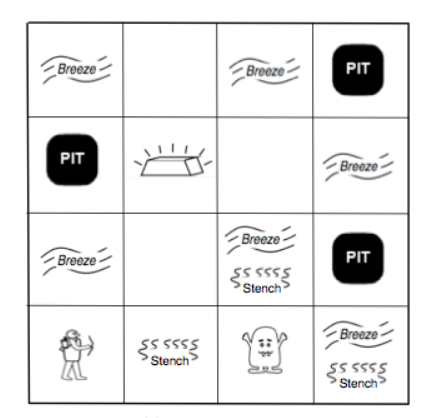
\includegraphics[scale=0.93]{wumpus}
    \caption{O Mundo do Wumpus}
    \label{fig:Figure1}
\end{figure}

\section{Estrutura Básica}

O código foi divido em quatro classes, presentes em quatro \emph{scripts} distintos, que representam as entidades envolvidas na exploração do mundo. A geração da configuração inicial de forma aleatória está presente na classe \textbf{WumpusWorld} (\emph{enviroment.py}). O armazenamento da base de conhecimento e o motor de inferência se encontram na classe \textbf{KnowledgeBase} (\emph{knowledge{\_}base.py}). A lógica de movimentação do agente está na classe \textbf{Explorarion} (\emph{movimentation{\_}logic.py}), e por fim, alguns métodos genéricos auxiliares foram implementados em um arquivo independente (\emph{utilities.py}).
    
\section{Implementação}

À seguir, serão detalhados de forma breve alguns aspectos que foram considerados de grande relevância no desenvolvimento desta implementação.

\subsection{Definição do Mundo e Restrições}

Embora o tamanho do ambiente possa ser alterado em código, inicialmente definimos o tamanho da malha como uma matriz 6 x 6, cuja matriz interna 4 x 4 corresponde às salas do mundo do Wumpus. As linhas e colunas 0 e 5 correspondem apenas às paredes do mundo como delimitadores. É importante citar que restringimos as posições adjacentes ao agente de conterem quaisquer poços ou Wumpus, já que isto forçaria o agente a tomar uma decisão aleatória (e sua possível morte), caso este recebesse uma percepção de \emph{Fedor} ou \emph{Brisa} em sua posição inicial. Vale citar que a valoração da medida de desempenho foi mantida como no enunciado.\\

\noindent Listaremos à seguir, as restrições que definimos na concepção do ambiente:

\begin{itemize}
    \item O agente sempre é colocado na posição (4, 1).
    \item Um poço e o Wumpus não podem ocupar a mesma posição.
    \item O agente e o ouro não podem ocupar a mesma posição inicialmente.
    \item O ouro pode estar em qualquer local que não esteja o agente ou poços, inclusive na mesma posição do Wumpus.\\
\end{itemize}

Ao final da construção do mundo, é atribuída à cada posição sua percepção, conforme a presença ou ausência de objetos adjacentes (acima, abaixo, direita, esquerda). As posições correspondentes aos limites do mundo, é aplicada somente a percepção de \emph{impacto}. Selecionamos como estrutura de dados uma \textbf{lista} para representar cada uma desta percepções, assim como sugerido no enunciado deste trabalho prático. É apresentado à seguir um exemplo desta representação:

\begin{center}
    \normalsize\textbf{['Nada', 'Brisa', 'Nada', 'Nada', 'Grito']}
\end{center}

\subsection{Movimentação do Agente}

Basicamente, o controle da movimentação fundamental do agente trabalha apenas com sua posição atual e anterior, assim como suas orientações (Cima, Baixo, Direita, Esquerda). O agente explorará o ambiente de forma contínua até o momento que uma das duas condições de paradas sejam satisfeitas. Estas condições são as seguintes:

\begin{itemize}
    \item O agente encontra o ouro.
    \item O agente estagna na busca pelo ouro, ou seja, visitou posições já exploradas anteriormente várias vezes consecutivas.
\end{itemize}

Dada a posição atual do agente, o ciclo básico de movimentação é obter todas as posições adjacentes ao mesmo, e então "perguntar" à base de conhecimento, qual a melhor ação que ele deve tomar, ou seja, para qual posição se deve ir.

Após atualizar as posições e orientações (anterior e atual) do agente, e realizar uma checagem de rotina se este ainda está vivo (caso a base de conhecimento direcione-o para um local com um poço ou Wumpus vivo), o agente obtém a percepção da sua posição atual e informa à base de conhecimento. Esta base irá analisar as percepções do agente, marcando possíveis posições perigosas, seguras, desconhecidas, além de inferir fatos, à medida que novas percepções são obtidas, dada a exploração do agente.

É importante citar que o controle das ações e pontuação do agente são incrementados à medida que este explora o ambiente, e que a manipulação das ações \emph{Girar}, \emph{Andar}, \emph{Agarrar} ocorre de forma conjunta com o auxílio dos métodos \emph{calculate\_action} e \emph{rotate\_180}, analisando as posições e orientações anteriores e atuais do agente, além de suas percepções.

No caso em que o agente ainda não encontrou o ouro e estagnou na exploração do ambiente por uma quatidade significativa de tempo, é optado por atirar a flecha no Wumpus, caso exista pelo menos uma posição suspeita de sua localização. No caso de haver mais de uma posição, o agente seleciona de forma aleaória o alvo, e em ambos os casos, a base de conhecimento é devidamente atualizada.

Se o Wumpus é morto, as percepções de Fedor deixam de existir, todas as posições marcadas como possível presença do mesmo, são identificadas como seguras (excetuando as que estejam marcadas como possíveis poços) e todas as percepções do mundo passam a apresentar o \emph{Grito}. Caso contrário, apenas a posição em que o agente atirou pode ser marcada como segura (novamente, excetuando possível poço) e o ambiente não é alterado.

\subsection{Base de Conhecimento}

O primeiro dever de nossa base de conhecimento é manter o controle dos locais que já foram visitados, e para isso, adicionamos os pares ordenados \((x, y)\) correspondentes às posições, à medida que o agente se movimenta pelo ambiente. Adicionamos também a posição atual à lista de posições seguras, já que o agente deve estar vivo para dizer suas percepções à base.

Após este controle, são realizadas as primeiras checagens. Primeiro checamos se o agente tentou se mover para uma parede, e caso afirmativo, a base recebe uma percepção de impacto e "diz" ao agente para retornar (girar 180° e mover-se para a posição anterior). A outra checagem de rotina é se a percepção atual indica \emph{Resplendor}, o que significa que o agente atingiu seu objetivo encontrando o ouro, não restando mais nada para fazer.

A partir deste ponto, começam as análises de maior importância realizando inferências, que serão entremamente relevantes na demarcação de possíveis perigos presentes no mundo. Para cada percepção enviada pelo agente, a base deverá analisá-la marcando locais com possíveis poços, possível Wumpus e locais seguros, conforme a presença ou ausência de percepções como: \emph{Fedor} e \emph{Brisa}.

\section{Execução e Saída}

Como mencionado anteriormente, utilizamos a biblioteca PyCryptodome para gerar pares ordenados aleatórios na construção do mundo, e em alguns casos, para retornar uma dentre várias ações seguras ou selecionar uma posição alvo para executar o disparo da flecha.\\

\noindent Para instalar, basta digitar o seguinte comando via terminal:

\begin{center}
    \boxed{\textbf{\normalsize{pip install pycryptodomex}}}
\end{center}

A execução do programa é feita em um \emph{script} separado (main.py) por motivos de organização, que importa todas as classes e métodos essenciais para execução do programa.\\

\noindent Para executar, basta digitar o seguinte comando via terminal:

\begin{center}
    \boxed{\textbf{\normalsize{python3 main.py}}}
\end{center}

Como saída, primeiramente o programa apresentará o mundo gerado e suas percepções, para então gerar o relatório dos dados armazenados na base de conhecimento a cada iteração (movimento do agente), que possui o seguinte formato padrão:

\begin{itemize}
    \item Posição atual
    \item Percepção atual
    \item Posições Desconhecidas
    \item Possíveis Poços
    \item Possível Wumpus
    \item Posições Seguras
\end{itemize}

É importante citar que a cada iteração, o programa pode exibir mensagens informando que o agente tentou mover-se para uma parede ou tentou atirar uma flecha (matando ou não o Wumpus) e, ao final da exploração, sempre é exibido se o ouro foi encontrado e a pontuação final obtida pelo agente.

\section{Limitações}

A implementação desenvolvida não possibilita ao agente ter noção da quantidade de poços ou Wumpus presentes no mundo, o que impede a base de conhecimento de realizar certas inferências probabilísticas. Priorizamos neste caso por sempre tomar uma ação que garanta a segurança do agente, portanto, observamos em nossos testes que a quantidade de vezes em que o agente estagnou durante a exploração do mundo foi ligeiramente maior do que as ocasiões em que este atingiu seu objetivo.

Podemos citar como exemplo a Figura \ref{fig:Figure2}, que apresenta casos em que um poço é posicionado em  (2, 1), o que é suficiente para o agente estagnar na exploração do mundo:

\begin{figure}[H]
    \centering
    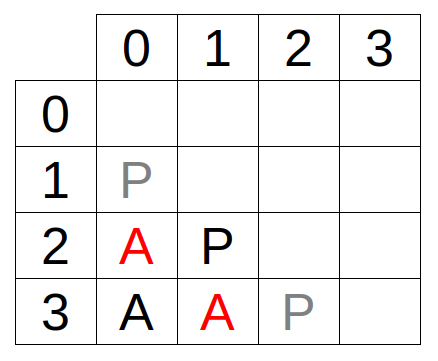
\includegraphics[scale=0.5]{deadlock.png}
    \caption{Agente se encontra em uma situação \emph{deadlock}}
    \label{fig:Figure2}
\end{figure}

Neste exemplo, o agente se moveria para as posições (2, 0) e (3, 1), obtendo como percepção uma \emph{Brisa} em ambas e marcando possíveis poços em (2, 0), (2, 1) e (3, 1), embora observando externamente, sabemos que um poço real só existe na posição (2, 1). Em situações como esta, o agente não tem garantia de segurança para continuar a explorar novas posições pelo mundo, restando como alternativa apenas uma escolha aleatória que pode levar a morte do mesmo, opção que não exploramos nesta implementação. A prioridade na tomada das ações é sempre buscar posições que garantam a segurança do agente, e por isso, ficar estagnado é muitas vezes inevitável.

\section{Conclusões}

Durante a implementação do trabalho, concordamos que a maior dificuldade encontrada foi a implementação do motor de inferências. Sempre avaliamos o mundo e suas percepções de modo que o agente tivesse condições de escolher o caminho mais seguro em busca de seu objetivo. 

Embora seja um problema de micro-mundo bastante "engessado" que apresenta um ambiente totalmente observável, os resultados que obtivemos confirmam a habilidade do agente, munido de sua base de conhecimento, a realizar a exploração e inferir conhecimento de acordo com a mesma. Em um ambiente diferente (com novos movimentos, componentes...), seria necessária uma fase adaptação para a construção de uma nova base de conhecimento para que o agente possa atuar de forma inteligente.

\section*{Referências}

\begin{itemize}
    \item Russell, Stuart; Norvig, Peter (2003). Articial Intelligence. A Modern Approach
(em inglês) 2a ed. Upper Saddle River, New Jersey: Prentice Hall.
    \item PyCryptodome Documentation: \url{https://pycryptodome.readthedocs.io/en/latest/index.html}
    \item Knowledge-base for Wumpus world: \url{https://python3.foobrdigital.com/knowledge-base-for-wumpus-world/}
\end{itemize}

\end{document}

